\PassOptionsToPackage{utf8}{inputenc}
\documentclass[12pt]{report}

\usepackage[margin=2cm]{geometry}

\usepackage{graphicx}

\renewcommand{\thefigure}{S\arabic{figure}}

\begin{document}

\begin{figure}[b]
	\centerline{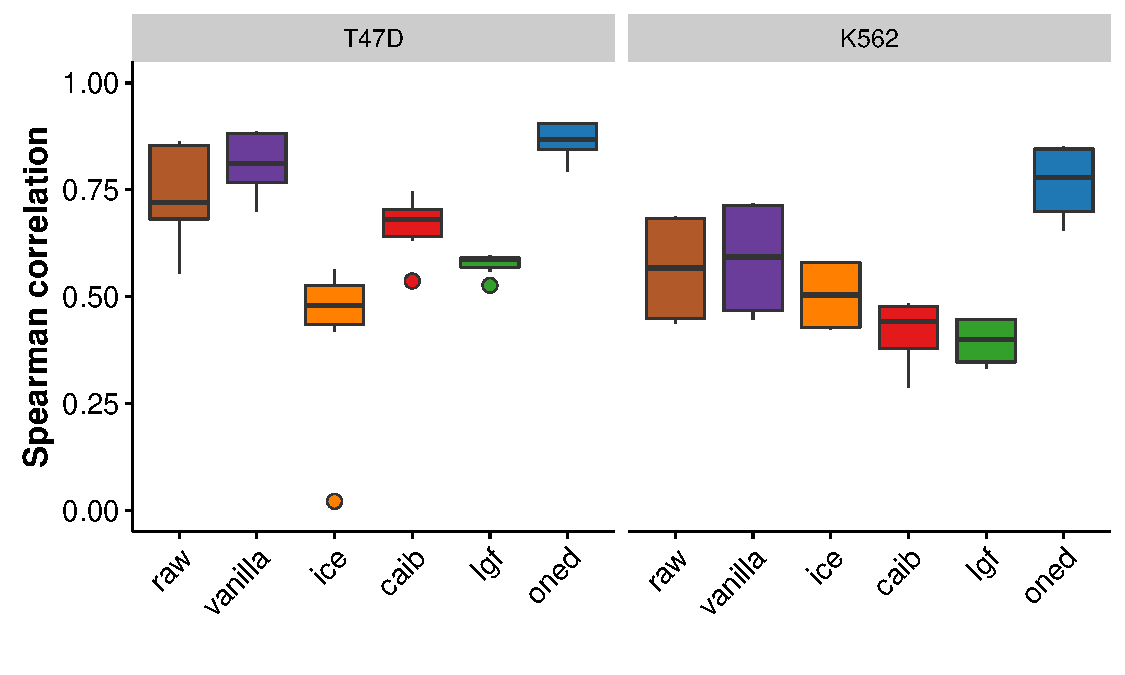
\includegraphics[width=\textwidth]{img/copy_number_suppfigure2.pdf}}
	\caption{
Spearman correlation between total number of contacts per bin and
independent copy number estimation (COSMIC) for each of the methods
compared. Left panel T47D breast cancer cell line, right panel K562
leukemia cell line. The new proposal (in blue) outperforms the rest of
alternatives.}
\end{figure}

\begin{figure}
\centerline{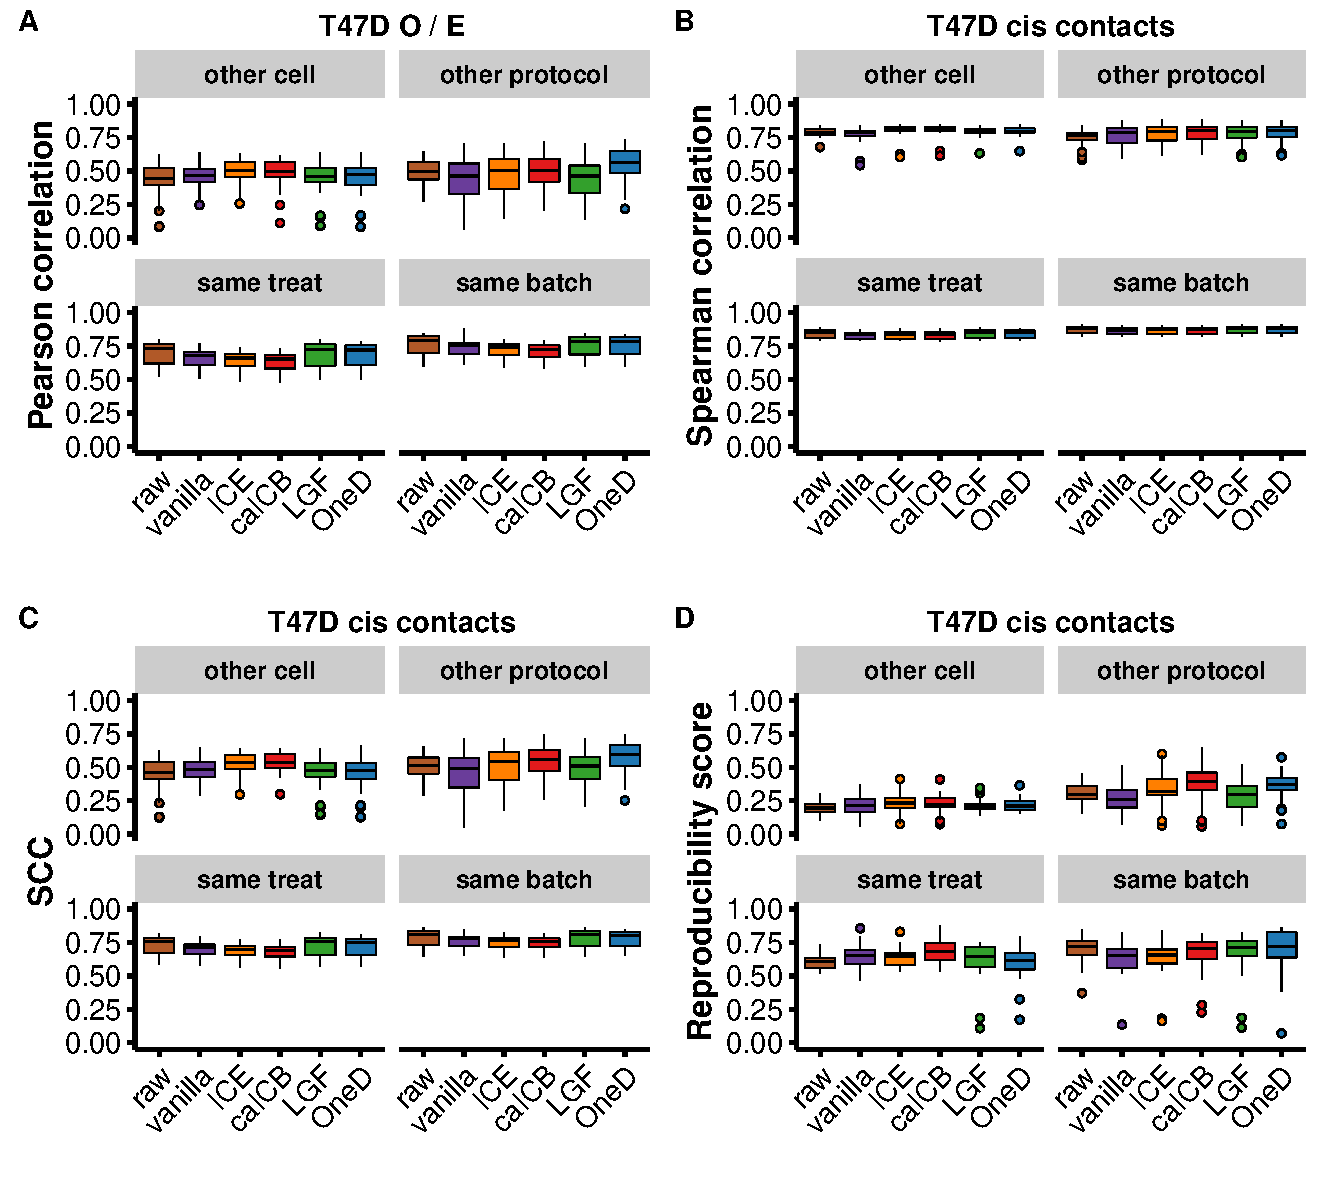
\includegraphics[width=\textwidth]{img/correlation_aberrant_boxplots1.pdf}}
\caption{Boxplots representing the results of the pair-wise comparisons of the
	samples included in the T47D set. X axis: different correction methods. Y
    axis: correlation. Each panel groups paris of samples with the correspondind
    characteristics (in terms of cell type, protocol, batch and
    treatment). A. Pearson correlation between observed over expected
    counts. B. Spearman correlation between observed counts. C. Stratum-adjusted correlation
    coefficient (SCC) between observed counts. D. Reproducibility score of
    observed counts.}
\end{figure}

\begin{figure}
\centerline{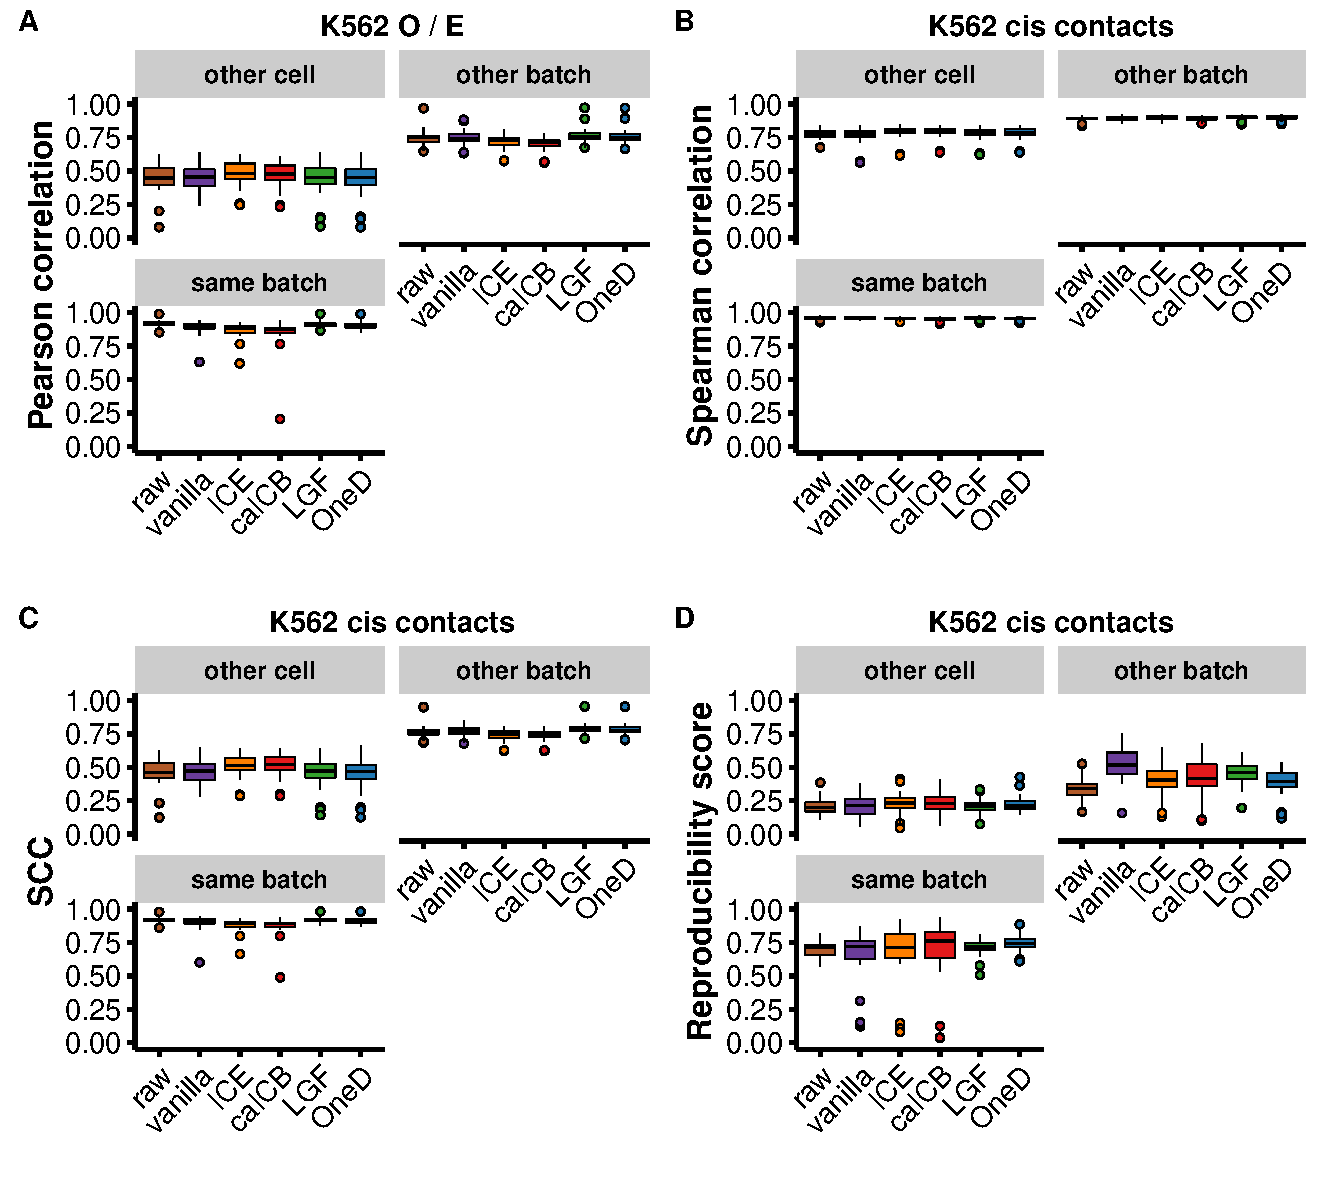
\includegraphics[width=\textwidth]{img/correlation_aberrant_boxplots2.pdf}}
\caption{Boxplots representing the results of the pair-wise comparisons of the
	samples included in the K562 set. X axis: different correction methods. Y
    axis: correlation. Each panel groups paris of samples with the correspondind
    characteristics (in terms of cell type, protocol, batch and
    treatment). A. Pearson correlation between observed over expected
    counts. B. Spearman correlation between observed counts. C. Stratum-adjusted correlation
    coefficient (SCC) between observed counts. D. Reproducibility score of
    observed counts.}
\end{figure}

\begin{figure}
\centerline{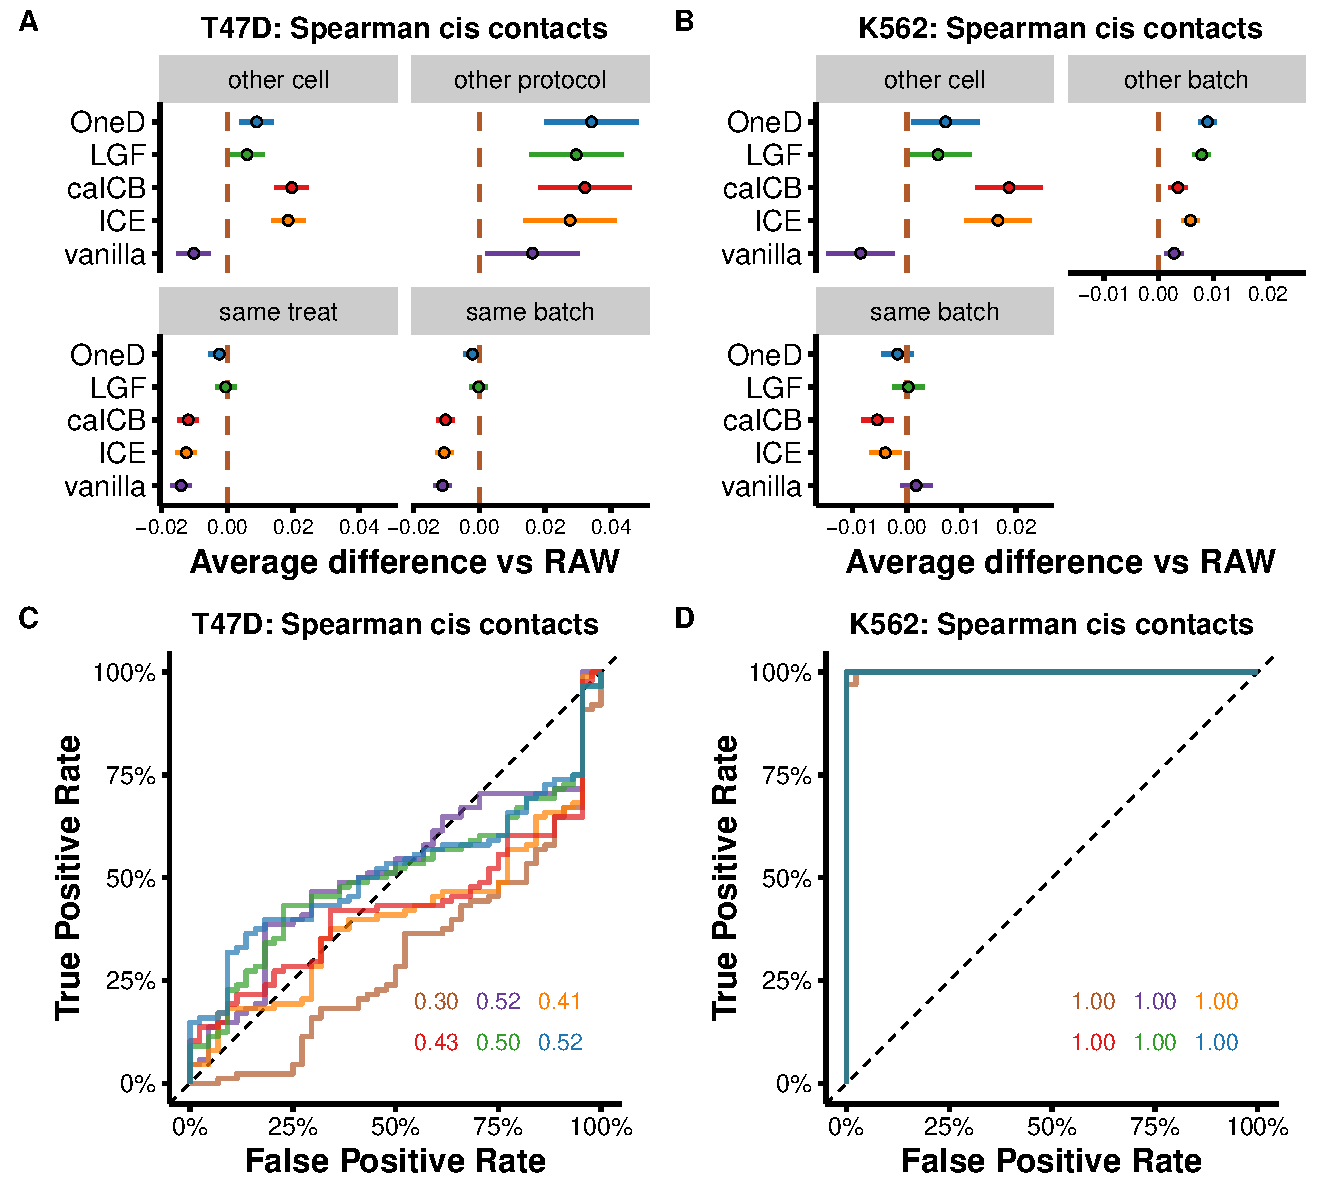
\includegraphics[width=\textwidth]{img/correlation_aberrant_spearman.pdf}}
\caption{
Results of the comparison between samples with aberrant karyotype. A and
B. Average changes compared to raw on the T47D and K562 sets. The bars
represent 95\% confidence intervals centered on the mean difference of the
correlation score between a given correction method and the raw data. The
brown dashed line indicates the value of the average score on raw matrices
(set to 0). C and D. ROC curves on the T47D and K562 sets. The areas under
the curve are indicated in the bottom right corner. The color code is the
same as panels A and B. The brown lines correspond to raw matrices. All
results in this figure are based on Spearman correlations between the
observed counts.}
\end{figure}

\begin{figure}
\centerline{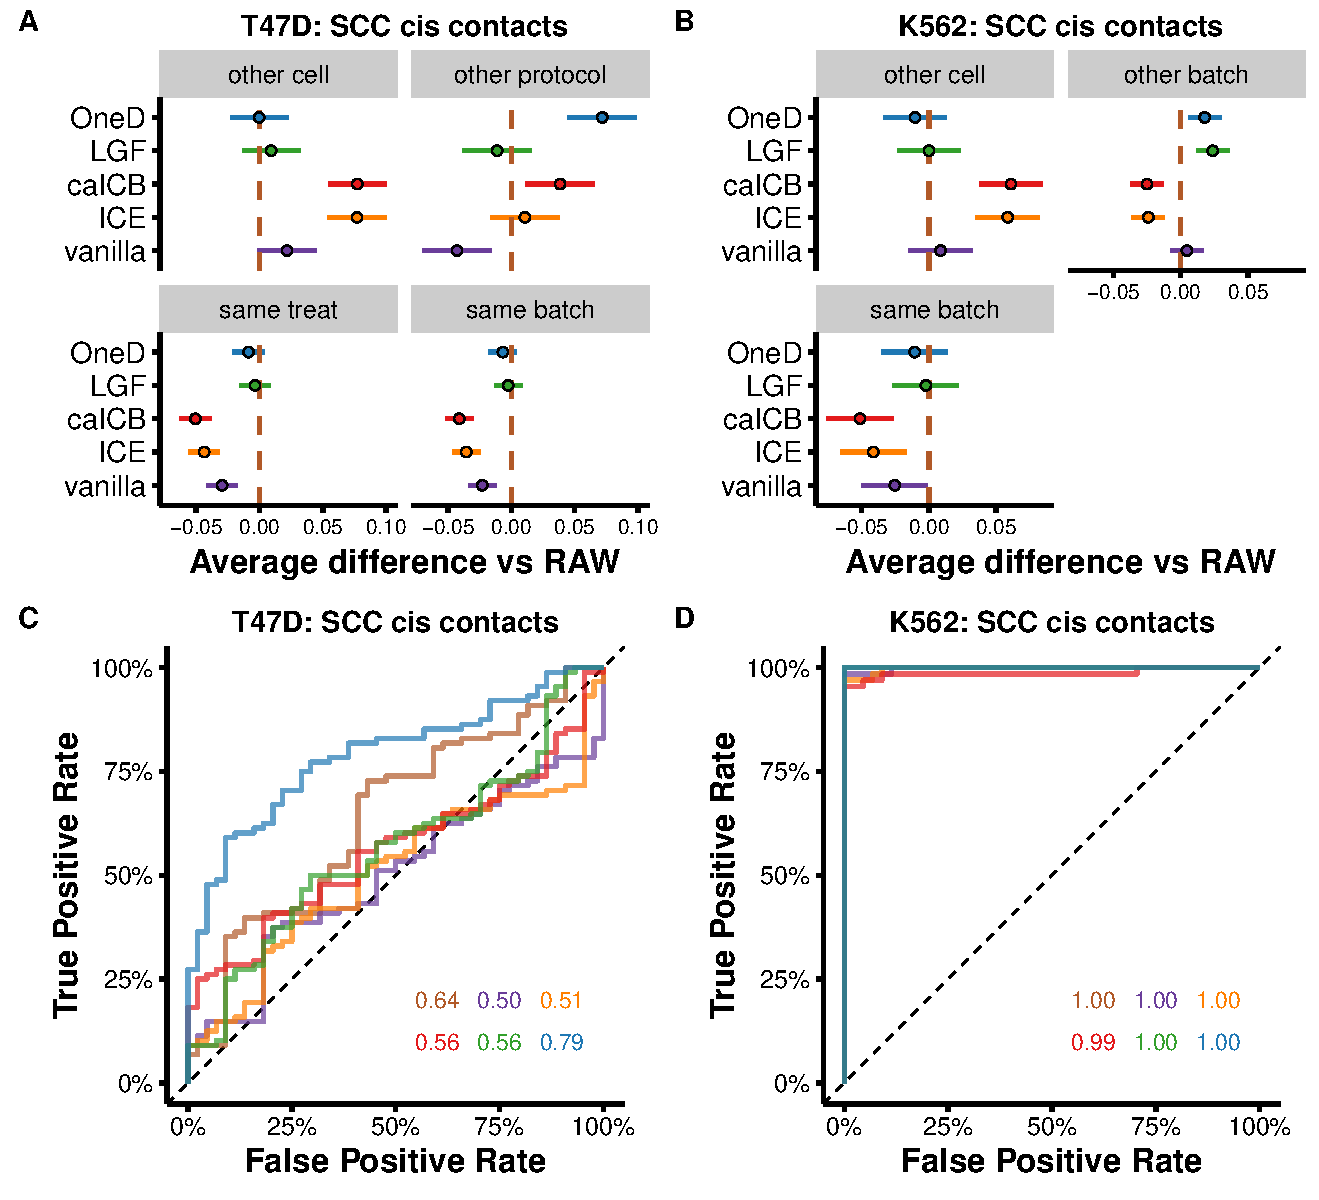
\includegraphics[width=\textwidth]{img/correlation_aberrant_scc.pdf}}
\caption{
Results of the comparison between samples with aberrant karyotype. A and
B. Average changes compared to raw on the T47D and K562 sets. The bars
represent 95\% confidence intervals centered on the mean difference of the
correlation score between a given correction method and the raw data. The
brown dashed line indicates the value of the average score on raw matrices
(set to 0). C and D. ROC curves on the T47D and K562 sets. The areas under
the curve are indicated in the bottom right corner. The color code is the
same as panels A and B. The brown lines correspond to raw matrices. All
results in this figure are based on stratum-adjusted correlations between the
observed counts.}
\end{figure}

\begin{figure}
\centerline{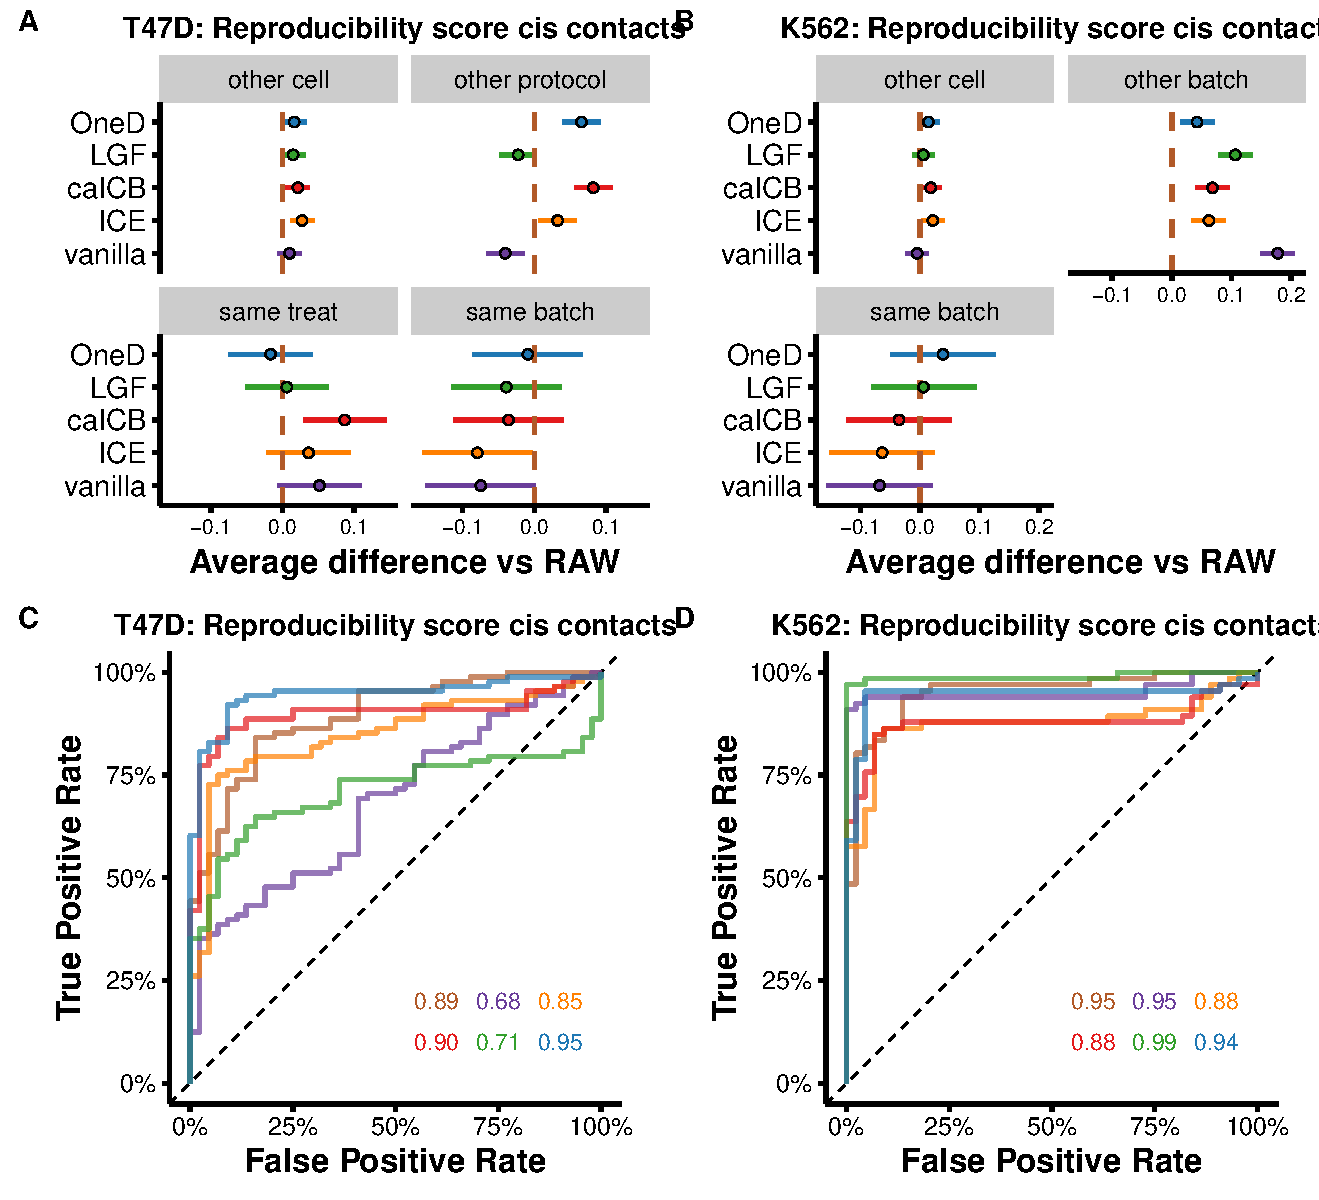
\includegraphics[width=\textwidth]{img/correlation_aberrant_repro.pdf}}
\caption{
Results of the comparison between samples with aberrant karyotype. A and
B. Average changes compared to raw on the T47D and K562 sets. The bars
represent 95\% confidence intervals centered on the mean difference of the
correlation score between a given correction method and the raw data. The
brown dashed line indicates the value of the average score on raw matrices
(set to 0). C and D. ROC curves on the T47D and K562 sets. The areas under
the curve are indicated in the bottom right corner. The color code is the
same as panels A and B. The brown lines correspond to raw matrices. All
results in this figure are based on the reproducibiliry score between the
observed counts.}
\end{figure}


\begin{figure}
\centerline{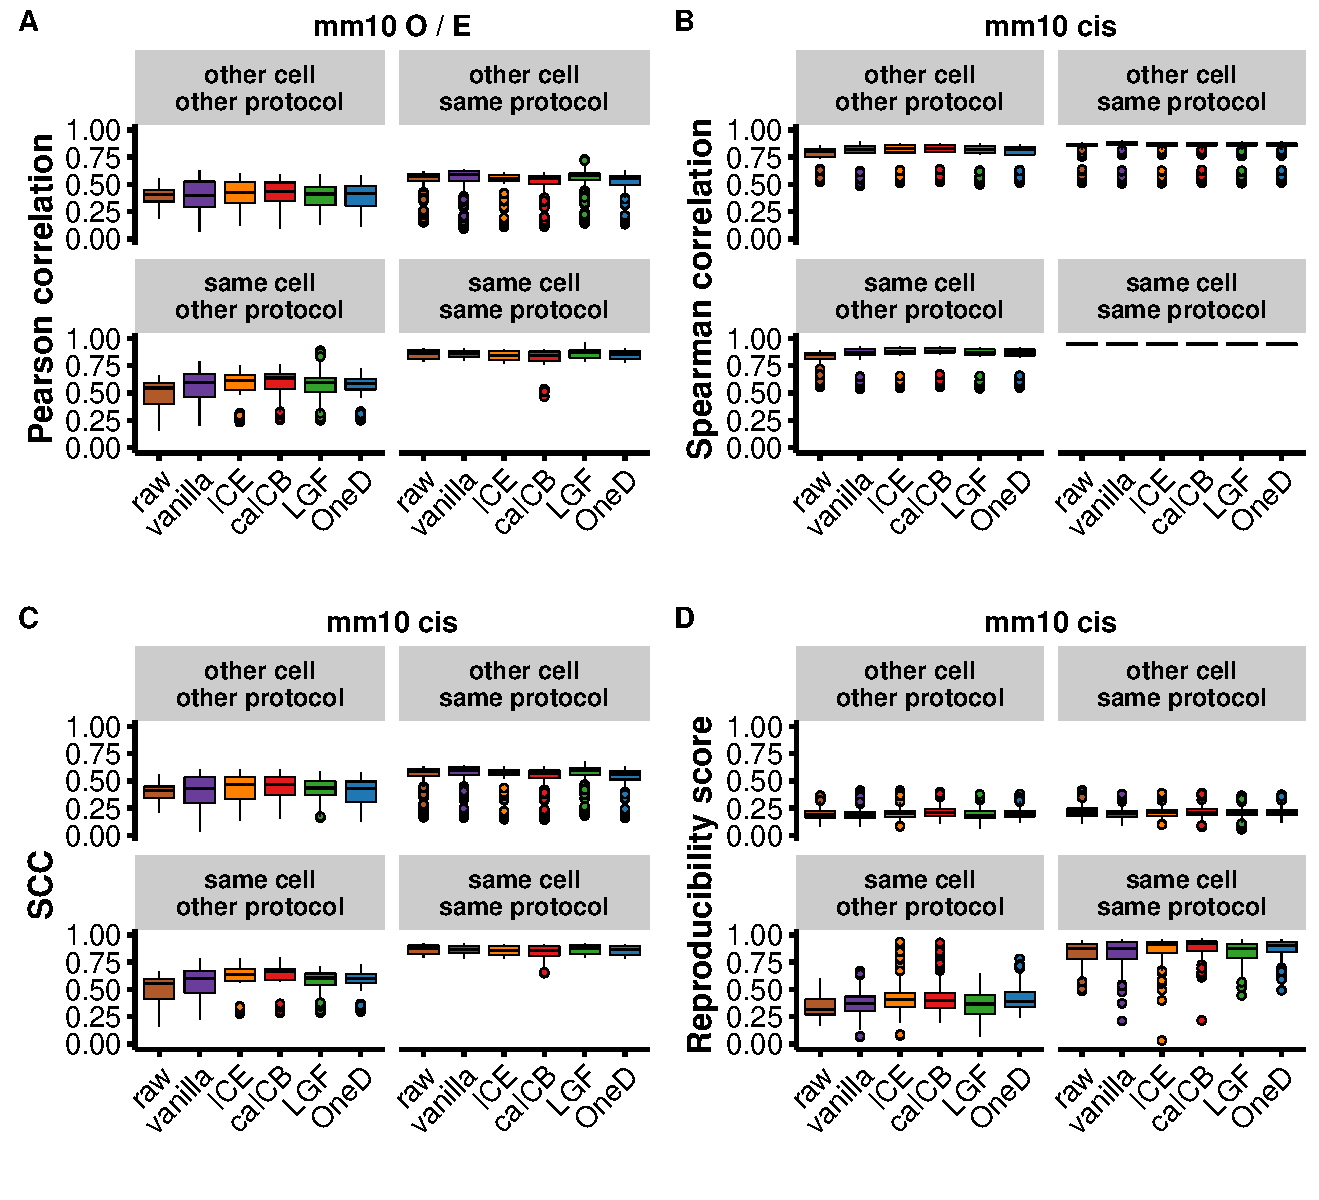
\includegraphics[width=\textwidth]{img/correlation_normal_boxplots.pdf}}
\caption{Boxplots representing the results of the pair-wise comparisons of the
	samples included in the mm10 set. X axis: different correction methods. Y
    axis: correlation. Each panel groups paris of samples with the correspondind
    characteristics (in terms of cell type, protocol, batch and
    treatment). A. Pearson correlation between observed over expected
    counts. B. Spearman correlation between observed counts. C. Stratum-adjusted correlation
    coefficient (SCC) between observed counts. D. Reproducibility score of
    observed counts.}
\end{figure}

\begin{figure}
\centerline{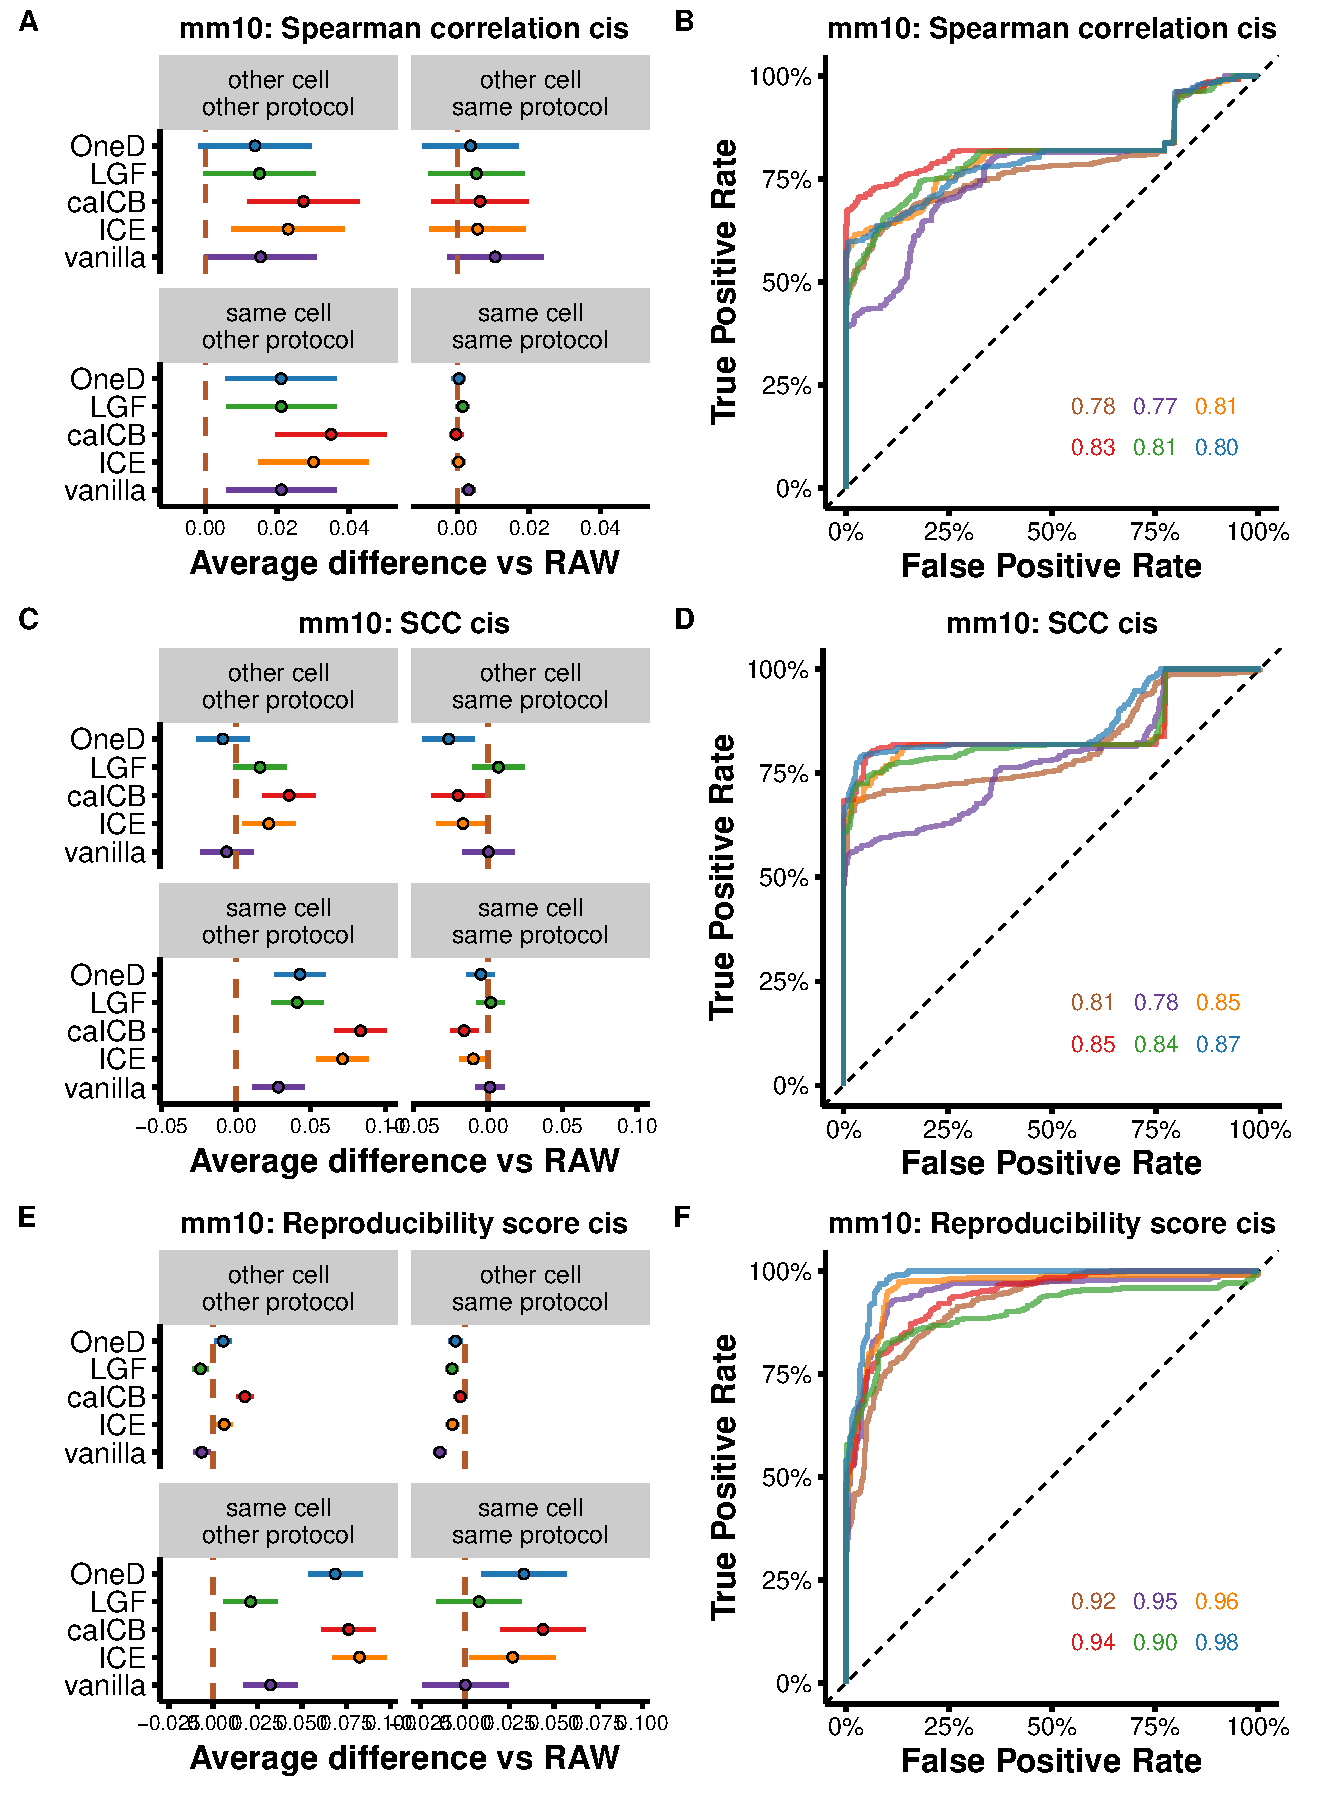
\includegraphics[width=.75\textwidth]{img/correlation_normal_other_metrics.pdf}}
\caption{Results of the comparison between samples with normal karyotype. A., C.
    and E.  Average changes compared to raw. The bars
represent 95\% confidence intervals centered on the mean difference of the
correlation score between a given correction method and the raw data. The
brown dashed line indicates the value of the average score on raw matrices
(set to 0). B., D. and F. ROC curves. The areas under
the curve are indicated in the bottom right corner. The color code is the
same as panels A, C. B. The brown lines correspond to raw matrices. Results in
panels A. and B. on Spearman correlations between the observed counts. Results in
panels C. and D. on Stratum-adjusted correlation coefficient (SCC) between observed counts. Results in
panels E. and F. on reproducibility score of observed counts.}
\end{figure}




\end{document}
